%-------------------------
% Resume in Latex
% Author : Aleksei Lapin
% Based off of: https://github.com/sb2nov/resume
% License : MIT
%------------------------
\documentclass[letterpaper,11pt]{article}
\usepackage[utf8]{inputenc}
\usepackage[T2A]{fontenc}
\usepackage[russian,english]{babel}
\usepackage{latexsym}
\usepackage[empty]{fullpage}
\usepackage{titlesec}
\usepackage{marvosym}
\usepackage[usenames,dvipsnames]{color}
\usepackage{verbatim}
\usepackage{enumitem}
\usepackage[hidelinks]{hyperref}
\usepackage{fancyhdr}
\usepackage{tabularx}
\usepackage{outlines}
\usepackage{ifthen}
\usepackage{xltabular}
\usepackage{graphicx}
\usepackage{fontawesome5} % icons
\input{glyphtounicode}
\usepackage[export]{adjustbox}
\usepackage{geometry}
\geometry{
  a4paper,
  top=20mm, 
  right=20mm, 
  bottom=15mm, 
  left=20mm
}

\pagestyle{fancy}
\fancyhf{} % clear all header and footer fields
\fancyfoot{}
\renewcommand{\headrulewidth}{0pt}
\renewcommand{\footrulewidth}{0pt}

% Adjust margins
\addtolength{\oddsidemargin}{-0.5in}
\addtolength{\evensidemargin}{-0.5in}
\addtolength{\textwidth}{1in}
\addtolength{\topmargin}{-.5in}
\addtolength{\textheight}{1.0in}

\urlstyle{same}

\raggedbottom
\raggedright
\setlength{\tabcolsep}{0in}

% Sections formatting
\titleformat{\section}{
  \vspace{-4pt}\scshape\raggedright\large
}{}{0em}{}[\color{black}\titlerule \vspace{-5pt}]

% Ensure that generate pdf is machine readable/ATS parsable
\pdfgentounicode=1

%-------------------------
% Custom commands
\newcommand{\resumeItem}[2]{
  \item\small{
    \textbf{#1}{: #2 \vspace{-2pt}}
  }
}

\newcommand{\resumeItemNoBold}[1]{
  \item\small{
    {\raggedright #1 \vspace{-2pt}}
  }
}

% Just in case someone needs a heading that does not need to be in a list
\newcommand{\resumeHeading}[4]{
    \begin{tabular*}{0.99\textwidth}[t]{l@{\extracolsep{\fill}}r}
      \textbf{#1} & #2 \\
      \textit{\small#3} & \textit{\small #4} \\
    \end{tabular*}\vspace{-5pt}
}

\newcommand{\resumeSubheading}[4]{
  \vspace{-1pt}\item
    \begin{tabular*}{0.97\textwidth}[t]{p{0.7\textwidth}@{\extracolsep{\fill}}r}
      \textbf{#1} & #2 \\
      \textit{\small\raggedright#3} & \textit{\small #4} \\
    \end{tabular*}\vspace{-5pt}
}

\newcommand{\resumeSubSubheadingItem}[3]{
  \vspace{-1pt}\item
    \begin{tabular*}{0.97\textwidth}{l@{\extracolsep{\fill}}r}
      \textbf{#1} | {#2} & \textit{\small #3} \\
    \end{tabular*}\vspace{-5pt}
}


\newcommand{\resumeSubSubheading}[2]{
    \begin{tabular*}{0.97\textwidth}{l@{\extracolsep{\fill}}r}
      \textit{\small#1} & \textit{\small #2} \\
    \end{tabular*}\vspace{-5pt}
}

\newcommand{\resumeSubItem}[2]{\resumeItem{#1}{#2}\vspace{-4pt}}

\renewcommand{\labelitemii}{$\circ$}

\newcommand{\resumeSubHeadingListStart}{\begin{itemize}[leftmargin=*]}
\newcommand{\resumeSubHeadingListEnd}{\end{itemize}}
\newcommand{\resumeItemListStart}{\begin{itemize}}
\newcommand{\resumeItemListEnd}{\end{itemize}\vspace{-5pt}}

\newcommand\clink[1]{{\usefont{T1}{lmtt}{m}{n} #1 }}

% Custom commands for awards with longer descriptions
\newcommand{\resumeAwardSubheading}[4]{
  \vspace{-1pt}\item
    \begin{tabular*}{0.97\textwidth}[t]{p{0.67\textwidth}@{\extracolsep{\fill}}r}
      \textbf{#1} & #2 \\
      \textit{\small\parbox[t]{0.67\textwidth}{\raggedright #3}} & \textit{\small #4} \\
    \end{tabular*}\vspace{-5pt}
}


%-------------------------------------------
%%%%%%  CV STARTS HERE  %%%%%%%%%%%%%%%%%%%%%%%%%%%%


\begin{document}

%----------HEADING-----------------
\begin{tabularx}{\linewidth}{@{}m{0.8\textwidth} m{0.2\textwidth}@{}}
    {
    \huge{\textbf{Алексей Лапин}} \newline
    \small{
        \clink{
            \href{mailto:a.lapin03@gmail.com}{\faEnvelope~\underline{a.lapin03@gmail.com}} \textbf{ | }
            {\fontdimen2\font=0.75ex \href{tel:+79217770608}{\faPhone~\underline{+7 (921) 777-06-08}}}\textbf{ | }
            \href{https://github.com/AaLexUser}{\faGithub~\underline{github.com/AaLexUser}}
        }
        \newline
        Санкт-Петербург, Россия
    }
    } &
    {
            \hfill
            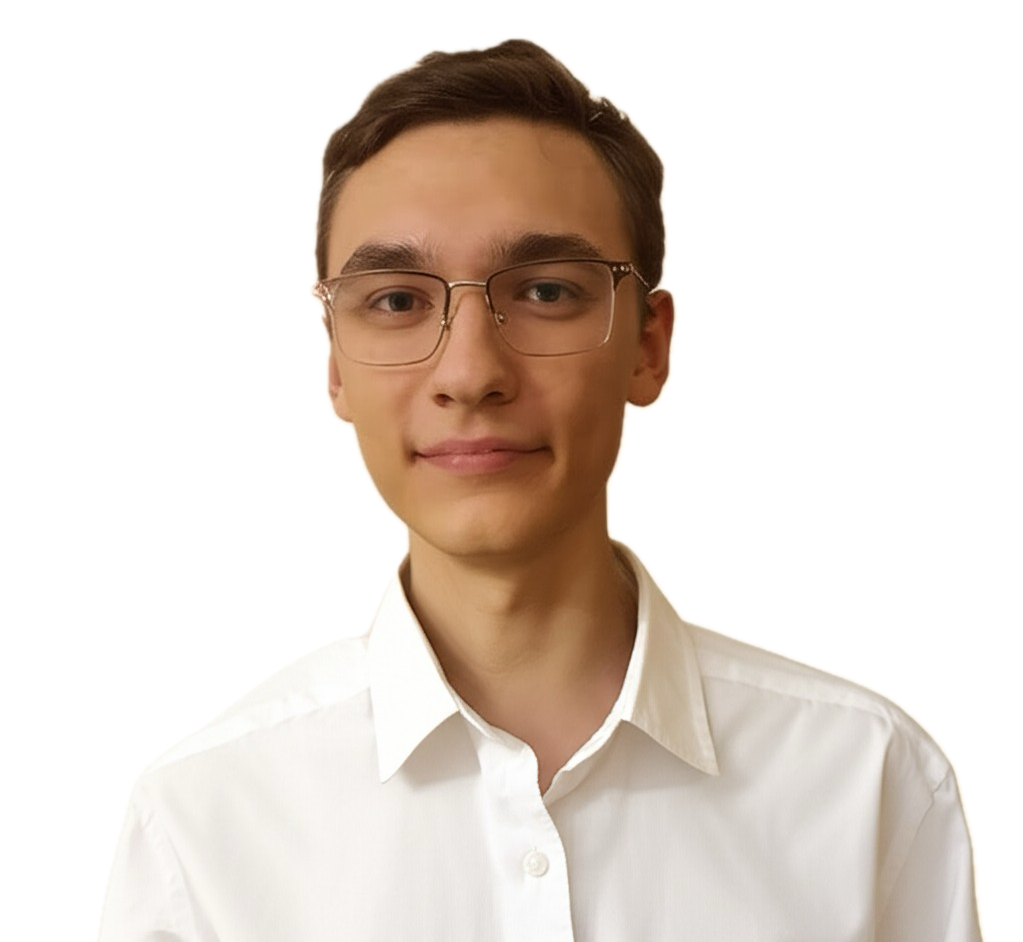
\includegraphics[width=2.8cm, frame]{../../photo/me.png}
        }
\end{tabularx}
\vspace{-25pt}

%-----------EDUCATION-----------------
\section{Образование}
\resumeSubHeadingListStart
\resumeSubheading
{\href{https://itmo.ru/}{Университет ИТМО}}{Санкт-Петербург, Россия}
{\href{https://abit.itmo.ru/program/bachelor/system_software}{Бакалавриат: Системное и прикладное программное обеспечение 09.03.04}}{Сентябрь 2021 -- Июль 2025}

\resumeSubItem{Relevant Coursework}{Системы искусственного интеллекта, Машинное обучение и анализ данных, Информационные системы и базы данных, Прикладная статистика, Теория вероятностей, Разработка сетевых приложений, Распределенные вычисления}
\resumeSubHeadingListEnd

%-----------JOB-----------------
\section{Опыт работы}
\resumeSubHeadingListStart
\resumeSubheading
{\href{https://aim.club/}{ИЦ ИТМО «Сильный искусственный интеллект в промышленности»}}{Санкт-Петербург, Россия}
{Лаборант}{Июля 2024 -- По настоящее время}
\resumeItemListStart
\resumeItemNoBold{Основной разработчик \textbf{мультиагентной} системы \textbf{автоматизированного машинного обучения} с применением \textbf{больших языковых моделей} – \href{https://github.com/aimclub/FEDOT.LLM}{\textbf{FEDOT.LLM}}.}
\resumeItemNoBold{\href{https://github.com/aimclub/FEDOT.LLM}{\textbf{FEDOT.LLM:}} \textbf{AutoML} следующего поколения с применением \textbf{БЯМ}. Он сочетает в себе мощь \textbf{больших языковых моделей} с \textbf{автоматизированными методами машинного обучения} для улучшения процессов \textbf{анализа данных} и \textbf{построения конвейеров}.}

\textbf{Технологии:} Python, NumPy, Pandas, Langchain, Streamlit, Chromadb, AutoML (FEDOT, FEDOT\_Ind, Autogluon), OpenAI.
\resumeItemListEnd
\resumeSubHeadingListEnd
%-----------PROJECTS-----------------
\section{Пет-Проекты}
\resumeSubHeadingListStart

\resumeSubheading{
    \href{https://github.com/AaLexUser/MyitmoGPT}
    {MyItmoGPT}}{\textit{Апрель 2024}}{Python, YandexGPT, Telegram Bot}{ }
\resumeItemListStart
\resumeItemNoBold{Телеграмм бот для получения расписания с my.itmo путем естественного разговора с YandexGPT.}
\resumeItemNoBold{Создал \textbf{промты} для \textbf{YandexGPT}, которые помогают извлекать нужную информацию из диалога с пользователем. Их ответом являются \textbf{аргументы для функции} в нужном формате. Это дало возможность получать необходимую информацию из внешних источников, недоступных LLM напрямую.}
\resumeItemNoBold{Написал \textbf{промты}, которые на основе данных из внешних источников и вопроса пользователя предоставляют точный и понятный ответ на интересующий вопрос.}
\resumeItemNoBold{Реализовал команды и ежедневные напоминания в \textbf{Telegram Боте}.}
\resumeItemListEnd

\resumeSubheading{
    \href{https://github.com/AaLexUser/Artificial-intelligence-systems}
    {Machine learning methods}}{\textit{Сентябрь - Ноябрь 2023}}{Python, ML, Scikit-learn} { }
\resumeItemListStart
\resumeItemNoBold{Реализованные модели: \textbf{линейная регрессия}, \textbf{метод k-ближайших соседей}, \textbf{деревья решений} и \textbf{логическая регрессия} - без использования внешних библиотек.}
\resumeItemNoBold{Модели использовались для анализа наборов данных, полученные метрики моделей сравнивались с метриками, полученными после обучения моделей \textbf{scikit-learn}.}
\resumeItemListEnd
\resumeSubHeadingListEnd

\section{Награды}
\resumeSubHeadingListStart
\resumeAwardSubheading{
    \href{https://drive.google.com/file/d/1gs8khjhjMai1iDpcuySTskslkZBpb5XG/view?usp=drive_link}
    {Хакатон AI Learning Lab}}{Санкт-Петербург, Россия}
{\textbf{Победитель}. Разработка платформы разметки данных для повышения качества обучения нейронных сетей.}{Февраль 2025}
\resumeAwardSubheading{
    \href{https://drive.google.com/file/d/1QIoI3PejwaDDYfFeW4Al2UtjX8WS3nBv/view?usp=drive_link}
    {XIV Конгресс молодых ученых ИТМО}}{Санкт-Петербург, Россия}
{\textbf{Победитель номинации "Лучший доклад молодого ученого"}. Проект "Разработка сервиса разметки данных для обучения нейронных сетей"}{Апрель 2025}
\resumeAwardSubheading{
    \href{https://drive.google.com/file/d/1w0LCMTmXbGLRT5wyzHR6HV2Q5f1fHShN/view?usp=drive_links}
    {XIV Конгресс молодых ученых ИТМО}}{Санкт-Петербург, Россия}
{\textbf{Победитель номинации "Лучший доклад молодого ученого"}. Проект "Разработка open-source инструмента автоматизированного машинного обучения с использованием больших языковых моделей"}{Апрель 2025}
\resumeSubHeadingListEnd

%--------PROGRAMMING SKILLS------------
\section{Технические навыки}
\resumeSubHeadingListStart
\resumeSubItem{Языки Программирования}{Clojure, Java, Python, SQL (PostgreSQL), TypeScript, C, C++}
\resumeSubItem{Фреймворки}{Spring Boot, Spring, Spring Data, Spring Security}
\resumeSubItem{Библиотеки}{React, Pandas, NumPy, Matplotlib, SFML}
\resumeSubItem{Инструменты разработчика}{Git, GitHub Actions, Gradle, Maven, Jupyter Notebook, GoogleCollab}
\resumeSubHeadingListEnd
\section{Дополнительная информация}
\resumeSubHeadingListStart
\resumeSubItem{Языки}{Английский язык -- B1}
\resumeSubHeadingListEnd
\end{document}
